%!TEX root = ../main.tex

\documentclass[../main.tex]{subfiles}
\begin{document}

\chapter{Introduction}
\label{chapter:introduction}

Our reliance on robots to keep our society functioning is increasing. As time goes on, more and more industries face changes in the technology landscape where the utilization of robots becomes a financial inevitability. This phenomenon drives the innovation that leads to smarter, cheaper, and more reliable robots. The proliferation of robots seems to fuel the automation of our daily lives where any task with minor repetitiveness is subject to automation. Some tasks like driving a car on the road or winning a game of Go, which were thought to be solvable only by humans, are already performed by computers equipped with some form of Artificial Intelligence. However, there are still a number of tasks that do not have satisfiable automated solutions. These tasks vary from safety critical tasks that directly impact lives to business operations tasks that determine profitability and efficiency of an organization.

Some examples of high impact tasks include search and rescue in the wilderness, natural disaster monitoring and relief, demining, and surveillance. Some examples of operations tasks are floor sweeping, factory automated painting, crop health monitoring, and ship hull inspection. The types of applications are broad but they all share a common theme. In fact, in its most general form, the problems described so far could all be stated as a coverage path planning problem.

The coverage path planing problem is a problem of computing a path for a robot such that the traversal of that path by the robot results in all points in the environment being under the robot's footprint as some point of time during the traversal. An example of a robot performing a coverage task is shown in Figure~\ref{img:example_coverage}. The problem is as old as the machine controlled milling. Only in 2000, Arkin\cite{arkin2000approximation} has demonstrated that the problem is in fact NP-complete. As such, there are numerous suboptimal solutions that have been proposed over the years. There are two surveys by Choset~\cite{choset2000coverage} and Galceran~\cite{galceran2013survey} that outline the most accepted solutions. Moreover, there is an extension to this problem that has been gaining popularity over the recent years. The use of multi robot systems for coverage to achieve better performance is becoming more appealing caused by decreasing cost of building robots.

\begin{figure}
	\centering
	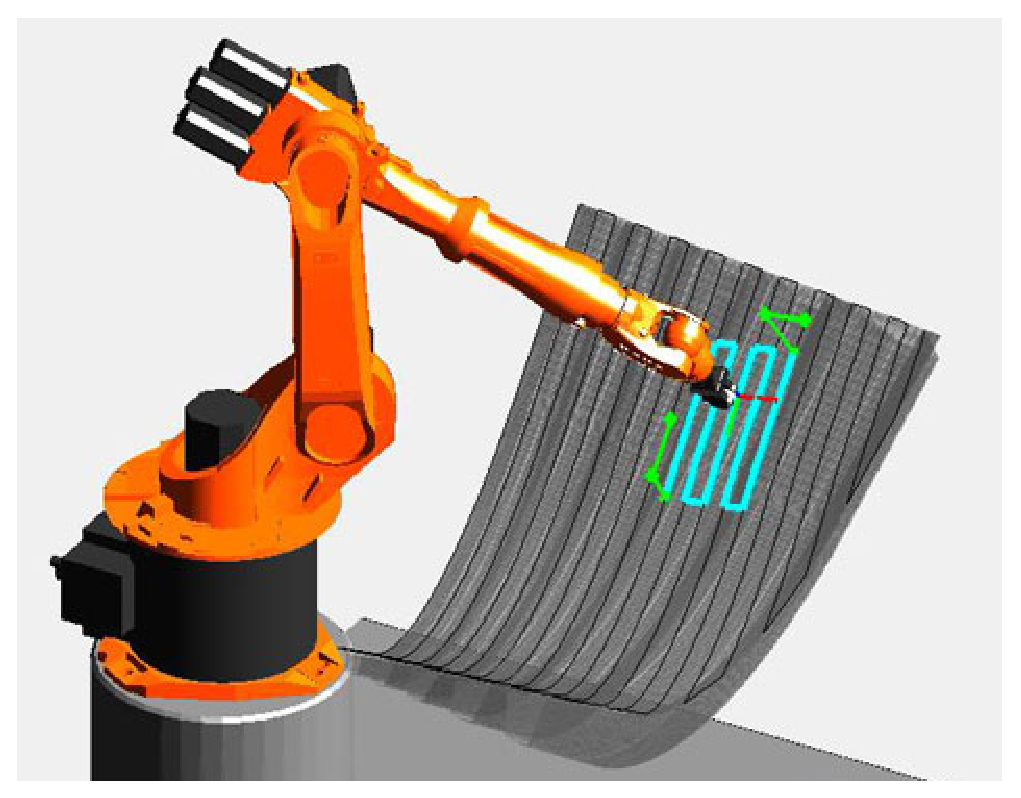
\includegraphics[scale=0.5]{img/chapter_1/example_coverage.eps}
	\vskip-15pt
	\caption*{\tiny twi-global.com}
	\caption{An example of an inspection coverage performed by a robotic arm.}
	\label{img:example_coverage}
\end{figure}

It is difficult to think about a good solution to the coverage path planning problem because the notion of \emph{goodness} varies from one application to another. For example, a good coverage path for a painting robot would result in the most uniform paint layer on the surface. A good coverage path for a monitoring application would result in the entire area observed in high quality. Because of this variety of metrics, the existing solutions in literature are typically very specialized. Other works in literature that focus on the theoretical analysis of the problem propose solutions that theoretically achieve complete coverage but in practice, are not feasible for any robot with the simplest of dynamics.

In this work, we propose an approach that aims to make coverage paths more usable in practice. We do this by structuring the paths generated by our method to be as \emph{straight} as possible. This is motivated by the typical dynamics of robots. Straight line segments are the simplest path segments that a robot can traverse. Vast majority of robotic systems are designed in a way that the traversal of a path between point $A$ and $B$ is the most efficient when this path is a straight line. In other words, we aim to compute paths with minimum number of turns. It should be noted that this goal can be achieved by minimizing the number of straight line segments required for complete coverage since every straight line segment has a turn associated with it to transition to the next straight line segment.

Our main contributions in this work are several. First, we design our own metric called the altitude that aids with the computation of the number of lines for full coverage. We then propose a greedy algorithm that partitions the workspace into regions with the minimum overall altitude. The result of the algorithm is a workspace partition with a set of lines. One of the important aspects of the algorithm is the procedure to make a minimum altitude cut dividing a polygon into two. We then solve the coverage problem by planning a tour of straight line segments by framing the problem is a Generalized Traveling Salesman Problem. We also provide proof of correctness of the algorithm as well the computational complexity analysis. Our final contribution is the extension of the single-agent coverage to the multi-agent case. We propose a partitioning scheme that divides the workspace into regions that results in comparable amount of work for each robot. The single robot coverage is then solved for each robot in the partition. 

\section{Relevant Works}
\label{sec:relevant_works}

The problem of coverage path planning sees many applications across numerous fields. The list includes applications like material polishing~\cite{rososhansky2010coverage}, autonomous farming~\cite{ollis1997vision}, de-mining~\cite{acar2003path}, floor cleaning~\cite{yasutomi1988cleaning}, and many others. Some of the earliest works in coverage could be traced to CNC trajectory planning works where operators would rely on experience and intuition to plan a trajectory for a tool. Perhaps one of the earliest works in literature is the work by Cao~\cite{cao1988region} where the authors outlines the requirement for a path to be a coverage path. There conditions state that all points must be covered, there should not be any overlap, all obstacles are to be avoided, and optimality is desired. These conditions are strict in that it is not always possible to fully satisfy them. However, this work set the stage for the research ahead.

One of the key contributions to the field of coverage is the work by Arkin~\cite{arkin2000approximation}. The authors have studied two variations of the coverage problem: the lawn mowing and milling. The difference is that milling problem does not allows the robot to cross the boundary of its workspace. The authors were able to show that these problems are in fact NP-hard, which suggests that the problem is computationally intensive with the size of the input. Some of the other problem related to coverage are the Travelling Salesman Problem, art gallery problem, and a watchman route problem.


There are various classifications use when talking about the coverage problem. Choset~\cite{choset2000coverage} have classified majority of the solutions to the problem by the methods used to discretized the environment. He summarized these to be either exact or approximate. However, there are a ton of other approaches that fall into the following categories as shown in the survey by Galceran~\cite{galceran2013survey}. These categories include: random and pseudo-random approaches, 3D coverage, coverage under uncertainty, persistent coverage, cooperative coverage, and others. In this section, we will cover some of the literature for single robot coverage.

The generation of an optimal coverage path for convex work spaces is tractable and can be solved efficiently using sweeping or spiralling motions. Minimum turn coverage for convex polygons has been considered in~\cite{maza2007multiple}. For general workspaces, the coverage problem is NP-hard~\cite{arkin2000approximation}. However, there are many approximate and heuristic approaches to coverage. One class of approaches is an \emph{exact} convex decomposition on the workspace in which the workspace is partitioned into convex regions. A coverage path consists of a tour of each region, with local coverage of a convex region performed with either sweeping or spiralling motion. Commonly-used methods for decomposition include Boustrophedon decomposition~\cite{Choset1998coverage}, its more general form, Morse-based decomposition~\cite{Acar2002morse}, and trapezoidal decomposition~\cite{Oksanen2009coverage}. Huang~\cite{Huang2001optimal} proposed a dynamic programming approach for generating a set of regions that minimize the number of turns in the overall coverage path. However, the runtime is exponential, and the cost associated with transitions between these regions is assumed to be negligible. Das~\cite{das2014mapping} used a greedy cut method for convex decomposition and computed a tour of the regions using a Traveling Salesman Problem (TSP) solver.

With exact decomposition, the quality of the coverage path is highly-dependent on the convex decomposition. For polygons without holes (obstacles), there are several suboptimal and optimal decomposition algorithms available~\cite{keil2000polygon}. Convex decomposition for polygons with holes is NP-hard~\cite{lingas1982power}. A drawback of exact decomposition is that for complex workspaces, the decomposition may contain many regions, resulting in large total transition costs between regions.

Another class of approaches is \emph{approximate} convex decomposition~\cite{Galceran2013surveycpp}, in which convex regions may overlap, and the union of regions approximates the workspace (points left uncovered are typically handled in a second pass). In the most common approach, each of the overlapping region is a coverage footprint, as shown in Figure~\ref{fig:footprints}(a). Local coverage of each region is ensured by visiting the region's center. Complete coverage becomes the problem of planning a tour that visits each center with minimum cost~\cite{arkin2000approximation}. A drawback of this method is that the overlap between regions reduces the efficiency of the overall coverage path. Also, the number of regions grows with the area of the workspace, making the problem of computing tours of the centers intractable for large spaces.




Paper with minimum turn TSP\cite{wagner2001approximation}
\cite{arkin2005optimal}.

There are many works that deal with multi-agent coverage. The concept of area coverage could be divided into classes. One has to be careful navigating the literature to pick the right class of coverage.

\textit{Sensor Coverage:}
The work by Durham~\cite{durham2012discrete} outlines a solution to the  multi-agent coverage under unreliable communication network. The environment is modeled as a grid with obstacles where the robots can move from one cell to another in the grid. The objective is to compute a partition that minimizes the coverage cost function. The computation of this function shares some similarities to Voronoi partitioning. The partitioning algorithm relies in pair-wise partitioning and reaches pair-wise optimality. The problem with this approach is that the environment as modeled as an occupancy grid. Also, this approach differs from ours as the robots is not requires to visit all cells; therfore, the cost function used in the optimization of the partition reflects that.

The work by Maza~\cite{maza2007multiple} proposed a solution to multi-agent coverage. Given $n$ robots, they partition the polygonal environment into $n$ regions. The partition is performed by anchored area partitioning algorithm. The area amount is reflective of the abilities of the robot. Once, the partition is formed, each robot cover their regions in an optimal sweeping fashion. The problems with the proposed approach is that the work only considered convex polygons. Furthermore, the assumption that the area alone reflects the abilities of the robot is too restrictive.

The work in \cite{barrientos2011aerial} have considered a similar problem with aerial drones. The divide the problem into three sections. First is the task allocation and the second is the path planning for each individual drone. The subregions are represented as a grid. This work shares a lot of similarities to the previous author but with extensive test trials.

Hokeyam~\cite{hokayem2007dynamic} worked on an algorithmic approach to coverage by robots following inner level sets of the polygonal workspace. Any collisions between robots are resolved by sporadic communications. The problem with using inner level sets of a polygon is that they make sense for convex polygons. However, for nonconvex polygons, some of these level sets become complicated. 

In another work~\cite{atincc2013supervised}, a control law for sensor coverage is developed for a team of robots that is based on gradient representation of coverage with the addition of the transition control law that helps the robots avoid local minima of gradients.

Another multi-robot visual coverage method developed by Valente~\cite{valente2011multi} where the approach is similar to our and that of Barrientos~\cite{barrientos2011aerial} where the robot divide the area via communications and plan the path accordingly. The assumption made here is that of convex polygon. One of the metric is the number of turns.

There are a number of works that study the coverage in a sense of sensor coverage. That is the problem becomes that of designing a control law that guides the robot to a location in the environment that maximizes some utility function%\cite{}. 




\end{document}